\documentclass[14pt]{extarticle}

\usepackage{fontspec}
\setmainfont{Times New Roman}

% размер полей
\usepackage{geometry}
\geometry{a4paper, top=2cm, bottom=2cm, right=1.5cm, left=3cm}

 %debugging
%\usepackage{showframe}

% полуторный интервал
\usepackage{setspace}
\onehalfspacing

% абзацный отступ
\setlength{\parindent}{1.25cm}

% выравнивание текста по ширине
\sloppy

% списки
\usepackage{calc} % арифметические операции с величинами
\usepackage{enumitem}
\setlist{
    nosep,
    leftmargin=0pt,
    itemindent=\parindent + \labelwidth - \labelsep,
}

% подписи к рисункам и таблицам
\usepackage{caption}
\renewcommand{\figurename}{Рисунок}
\renewcommand{\tablename}{Таблица}
\DeclareCaptionFormat{custom}
{
    \textit{#1#2#3}
}
\DeclareCaptionLabelSeparator{custom}{. }
\captionsetup{
    % хз какой это размер - 12 или нет, но выглядит меньше 14
    font=small,
    format=custom,
    labelsep=custom,
}

% картинки
\usepackage{graphicx}

% колонтитулы
\usepackage{fancyhdr}

% картинки и таблицы находятся именно в том месте текста где помещены (атрибут H)
\usepackage{float}

% таблицы
\usepackage{tabularray}

\graphicspath{ {6.3.3/models/} }
\begin{document}
\pagestyle{fancy}
\fancyhead{}
% disable header
\renewcommand{\headrulewidth}{0pt}
\fancyfoot[L]{Дубровских гр 221-361}
\fancyfoot[C]{ЛР 6.3.3}
\fancyfoot[R]{Продажа автотранспорта}
\singlespacing

\newpage
\begin{center}
    Министерство науки и высшего образования Российской Федерации
    Федеральное государственное автономное образовательное учреждение

    высшего образования

    \guillemotleft МОСКОВСКИЙ ПОЛИТЕХНИЧЕСКИЙ УНИВЕРСИТЕТ\guillemotright

    (МОСКОВСКИЙ ПОЛИТЕХ)
\end{center}
\noindent
\bigbreak
\bigbreak
\bigbreak
\bigbreak
\begin{center}
    ЛАБОРАТОРНАЯ РАБОТА 6.3.3

    По курсу Проектирования пользовательских интерфейсов в веб

    \textbf{Выбор и оптимизация цветовых палитр сайта}
    \bigbreak
    \bigbreak
    \bigbreak
    \bigbreak
    ТЕМА

    \guillemotleft\textbf{САЙТ ДЛЯ ПРОДАЖИ И ПОИСКА АВТОМОБИЛЕЙ}\guillemotright
\end{center}
\noindent
\bigbreak
\bigbreak
\bigbreak
\bigbreak
\bigbreak
\bigbreak
\bigbreak
\bigbreak
\bigbreak
\bigbreak
\hfill Выполнил

\hfill Дубровских Никита Евгеньевич

\hfill Группа 221-361
\bigbreak
\bigbreak
\bigbreak
\hfill Проверил

\hfill Натур ВВ
\vfill
\begin{center}
    Москва, 2024
\end{center}
\newpage
\onehalfspacing


\begin{center}
    \textbf{Лабораторная работа 6.3.3}

    \textbf{Выбор и оптимизация цветовых палитр сайта}
\end{center}

\textbf{Цель работы:} выбрать, оценить и оптимизировать цветовую гамму (палитру) пользовательского интерфейса с учетом аномалий цветового восприятия пользователей и возможности цветовоспроизведения экранного
\bigskip

\textbf{Задачи:}

\begin{enumerate}
    \item Выбрать мудборд для интерфейса и извлечь палитру. 
    \item Выбрать (сгенерировать) цветовую (ые) палитру (ы) пользовательского интерфейса веб-сайта (мобильного приложения)
    \item Провести анализ цветовой гаммы (палитры) пользовательского интерфейса с учетом аномалий цветовосприятия пользователей веб-сайта (мобильного приложения), внести необходимые коррективы.
    \item Провести анализ цветовой гаммы (палитры) пользовательского интерфейса с учетом экранного цветовоспроизведения по таблице «безопасных» веб-цветов, внести необходимые коррективы.
    \item Зафиксировать оптимальный вариант цветовой гаммы (палитры) с указанием названий цветов и их описанием в различных цветовых системах.
    \item С помощью сервисов разработать пример веб-страницы в созданной палитре.
\end{enumerate}
\bigskip

\textbf{Основные термины}

\begin{itemize}
    \item Цветовая палитра - набор цветов, используемых в интерфейсе веб-сайта или мобильного приложения.
    \item Мудборд - коллаж изображений, отражающих настроение и концепцию визуального продукта.
    \item Аномалии цветовосприятия - нарушения восприятия цветов, которые могут влиять на пользователей.
    \item Экранное цветовоспроизведение - способность экранов воспроизводить цвета, которые могут отличаться от реальных.
    \item RGB - модель цвета, основанная на комбинации красного, зеленого и синего.
    \item HSB/HSV - модели цветового пространства, описывающие цвета в терминах оттенка, насыщенности и яркости.
    \item Контрастность - разница между светом и темнотой цветов, важная для доступности.
    \item Генератор палитр - онлайн-инструмент для создания и оптимизации цветовых палитр.
    \item Безопасные веб-цвета - набор цветов, которые гарантированно отображаются одинаково на всех устройствах и браузерах.
\end{itemize}
\bigskip

\textbf{Ассоциации, эмоции, предметы, цвета}
\bigskip

Ассоциации:
\begin{itemize}
    \item скорость – ощущение свободы, путешествий, динамики;
    \item престиж – статус, стиль, роскошь;
    \item независимость – возможность самостоятельного перемещения, личная свобода;
    \item мощь и сила – особенно ассоциируется с мощными спорткарами и внедорожниками.
\end{itemize}
\bigskip

Эмоции:
\begin{itemize}
    \item волнение – особенно на высокой скорости или в спорткаре;
    \item спокойствие и комфорт – особенно в просторных, удобных автомобилях;
    \item приключение – чувство готовности к дальним поездкам и исследованию новых мест;
    \item радость и удовольствие – наслаждение от управления автомобилем и свободы движения.
\end{itemize}
\bigskip

Предметы:
\begin{itemize}
    \item руль;
    \item шины;
    \item фары;
    \item ключи;
    \item панель управления;
    \item зеркала;
\end{itemize}
\bigskip

Цвета:
\begin{itemize}
    \item красный – энергия, страсть, скорость;
    \item синий – спокойствие, надежность;
    \item черный – роскошь, мощь, престиж;
    \item белый – чистота, стиль, минимализм;
    \item серебристый и серый – технологичность, классика, нейтральность.
\end{itemize}
\bigskip

\noindent
\begin{minipage}{\linewidth}
    \fbox{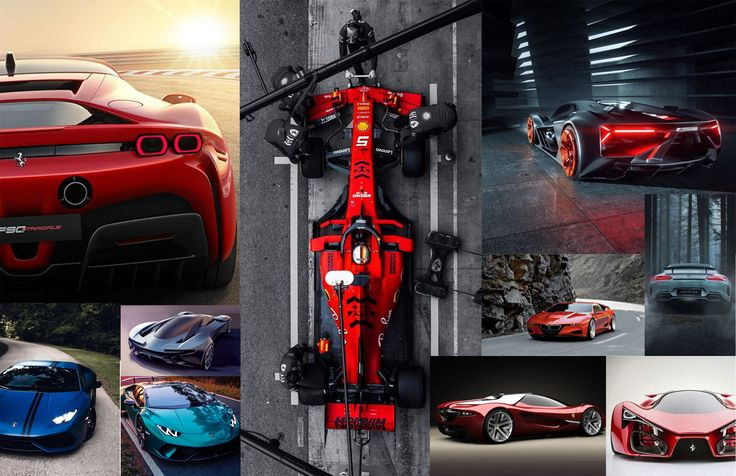
\includegraphics[width=\linewidth]{moodboard3}}
    \captionof{figure}{Мудборд}
\end{minipage}
\bigskip

\noindent
\begin{minipage}{\linewidth}
    \fbox{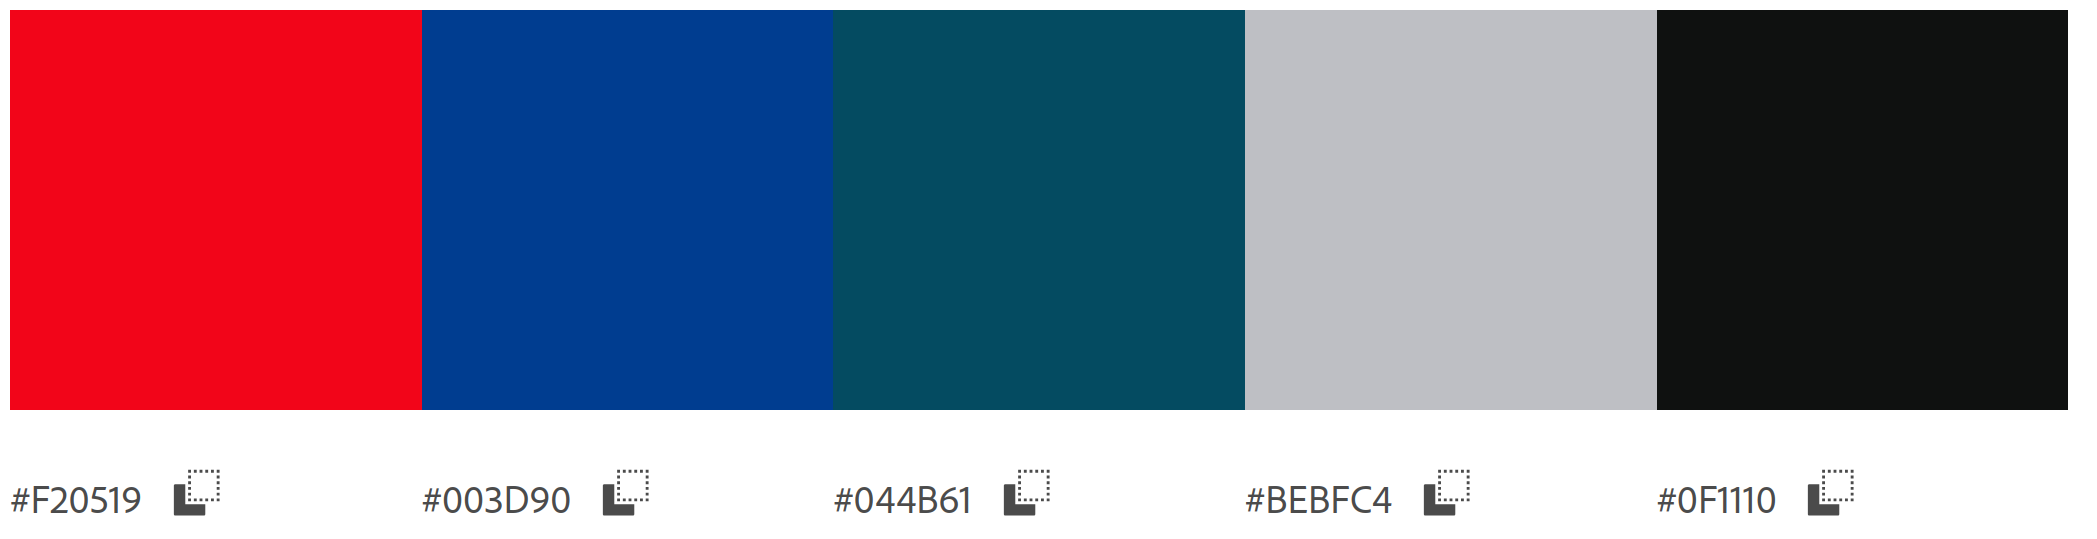
\includegraphics[width=\linewidth]{moodboard3_pallete}}
    \captionof{figure}{Палитра мудборда}
\end{minipage}
\bigskip

На мудбордах преимущественно присутствуют цвета: красный, черный, синий, белый.
\bigskip

\noindent
\begin{minipage}{\linewidth}
    \fbox{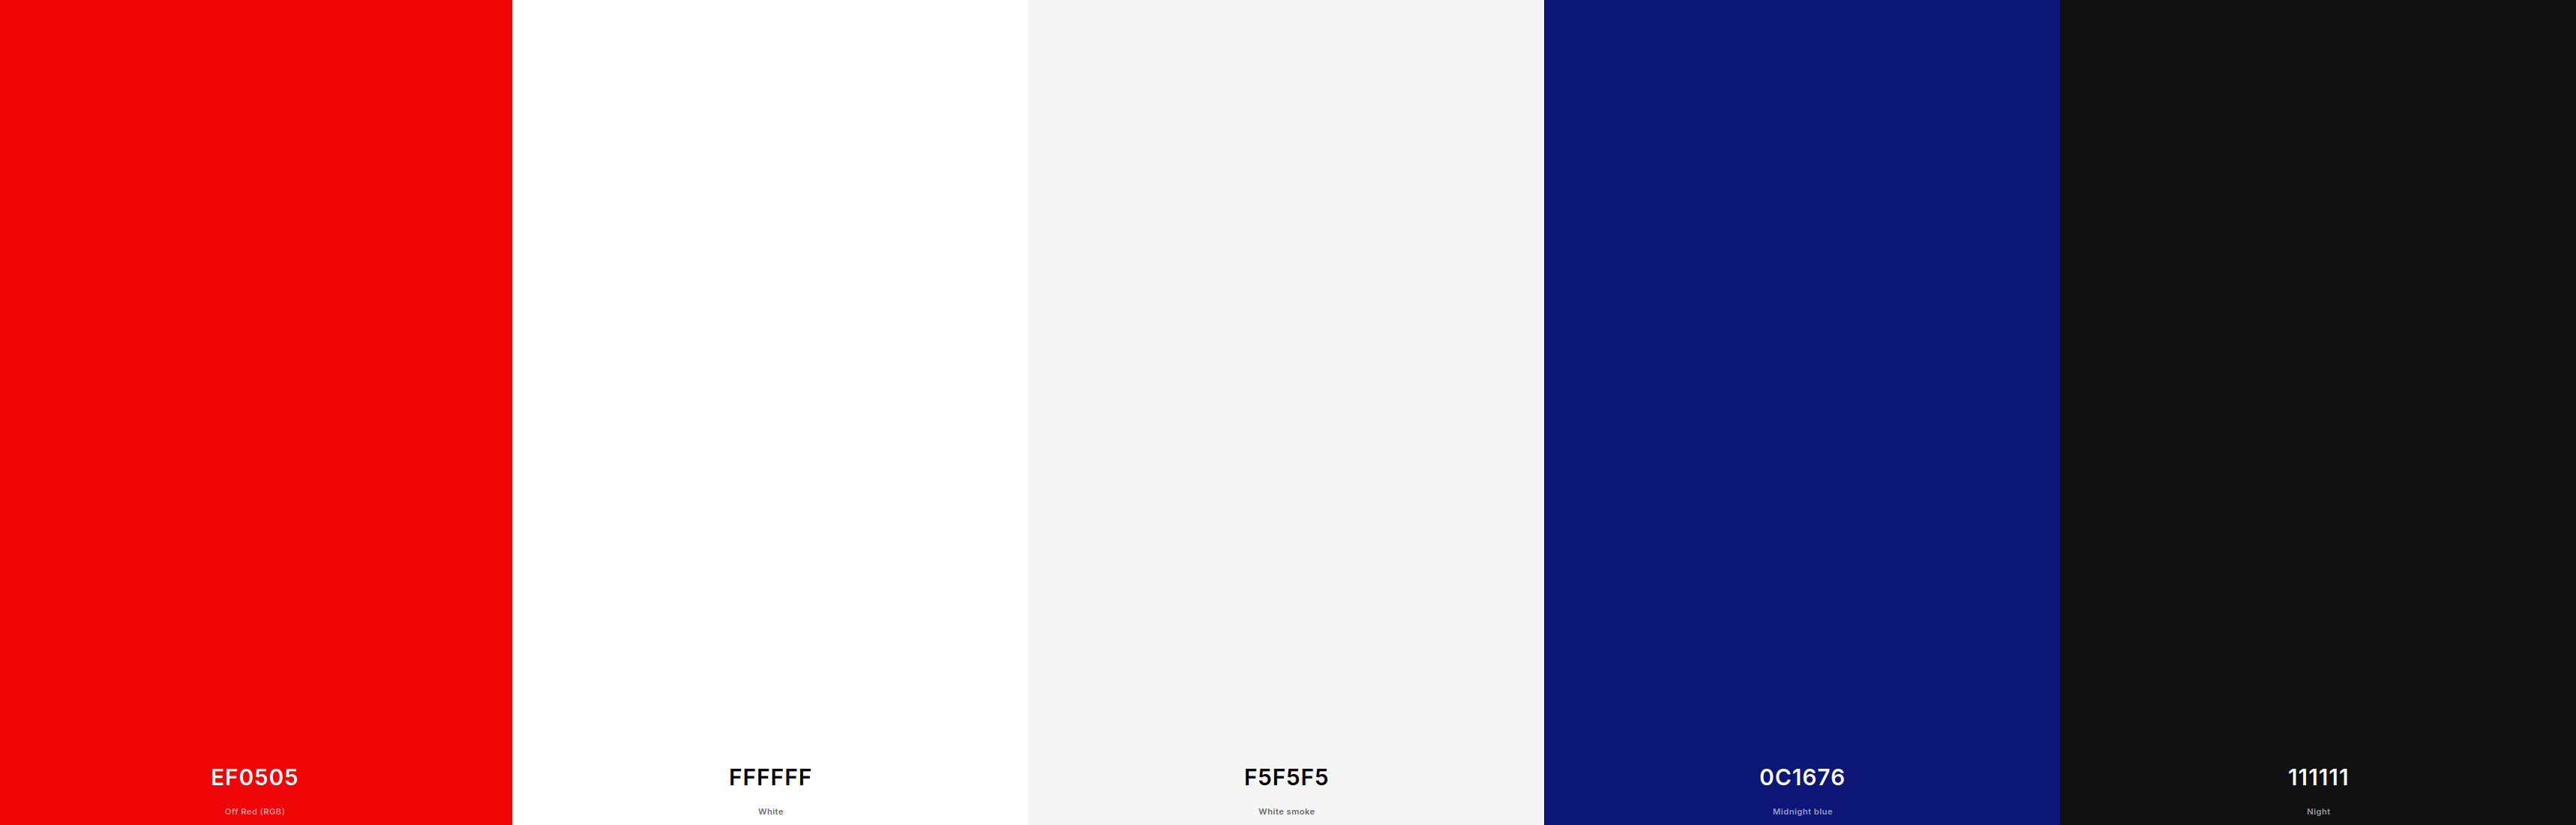
\includegraphics[width=\linewidth]{coolors5}}
    \captionof{figure}{Палитра сгенерированная в сервисе coolors.co}
\end{minipage}
\bigskip

\noindent
\begin{minipage}{\linewidth}
    \fbox{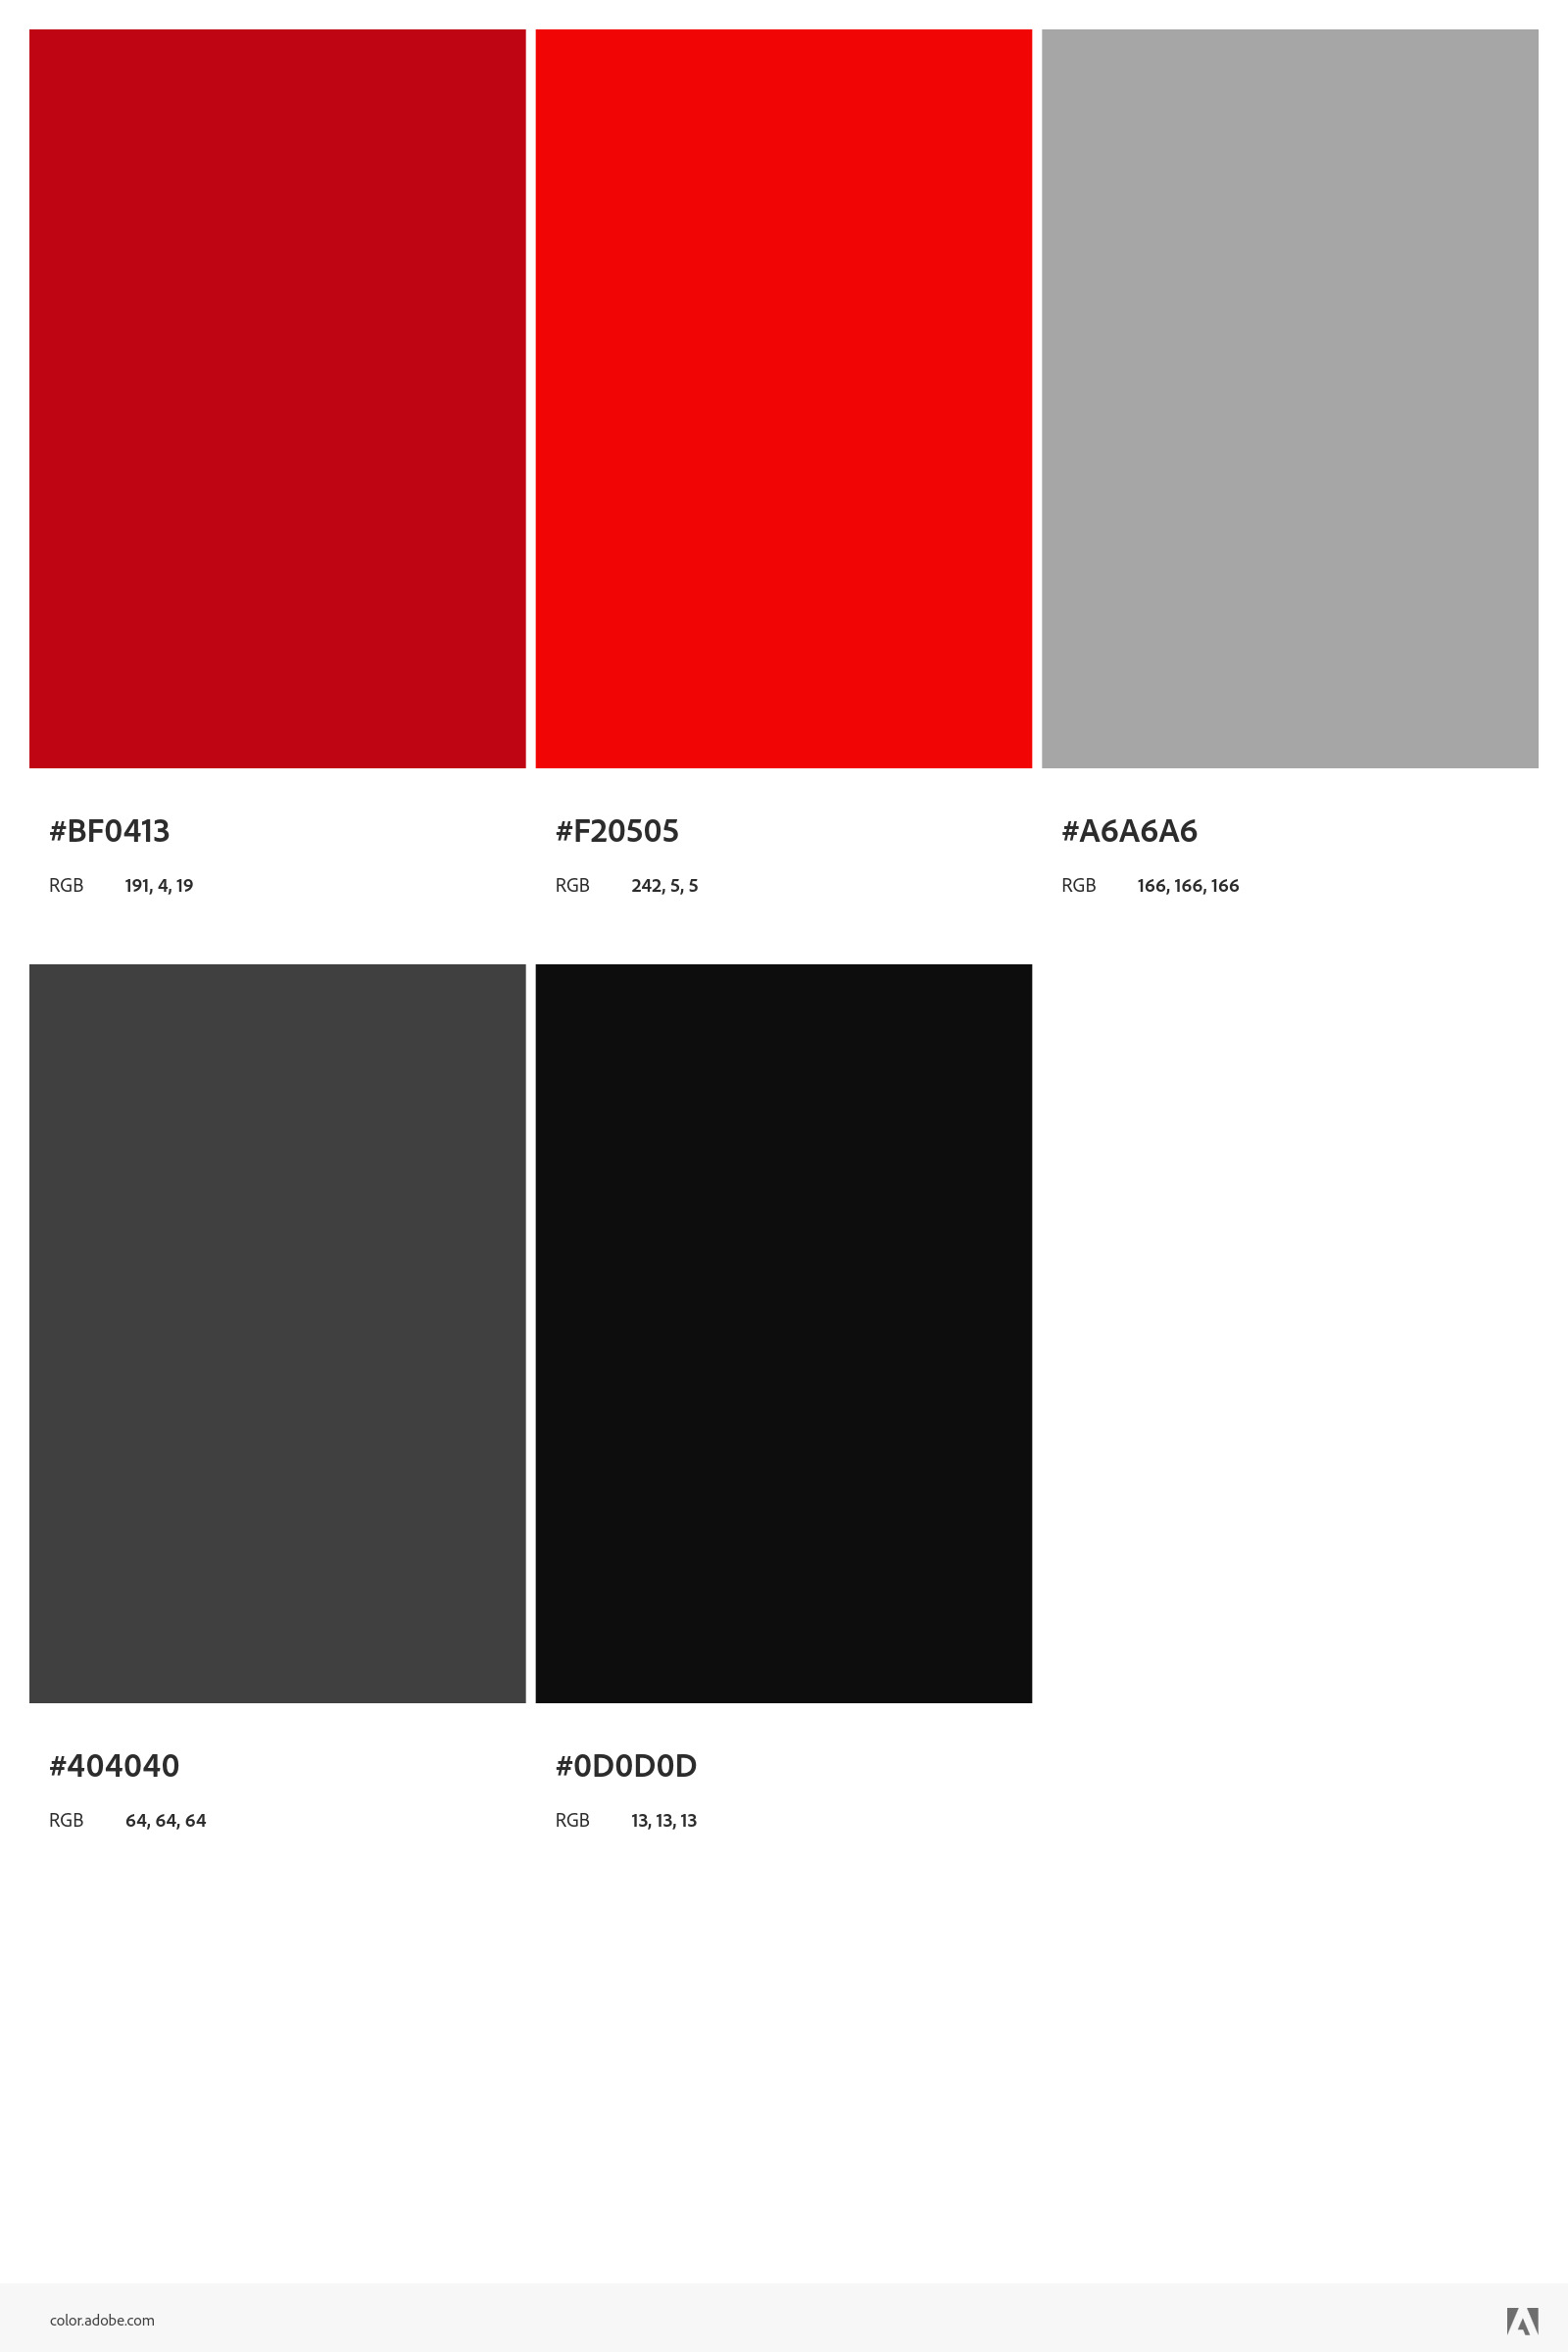
\includegraphics[width=\linewidth]{adobe}}
    \captionof{figure}{Палитра сгенерированная в сервисе color.adobe.com}
\end{minipage}
\bigskip

\noindent
\begin{minipage}{\linewidth}
    \fbox{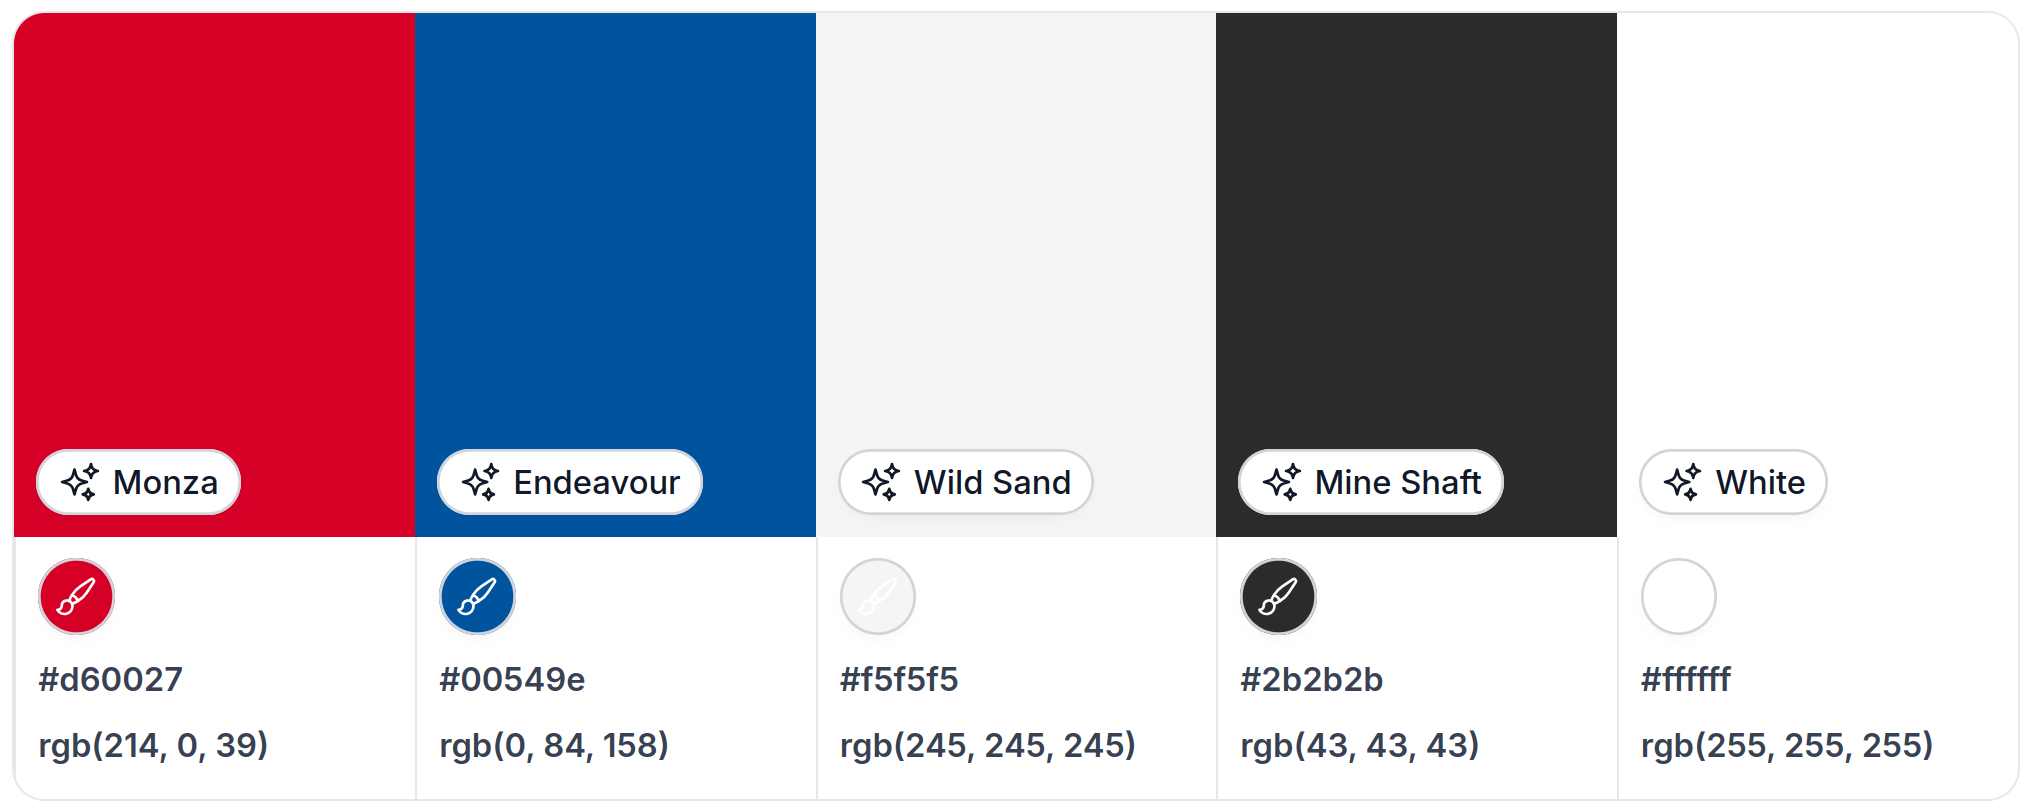
\includegraphics[width=\linewidth]{colormagic}}
    \captionof{figure}{Палитра сгенерированная в сервисе colormagic.app}
\end{minipage}
\bigskip

\noindent
\begin{minipage}{\linewidth}
    \fbox{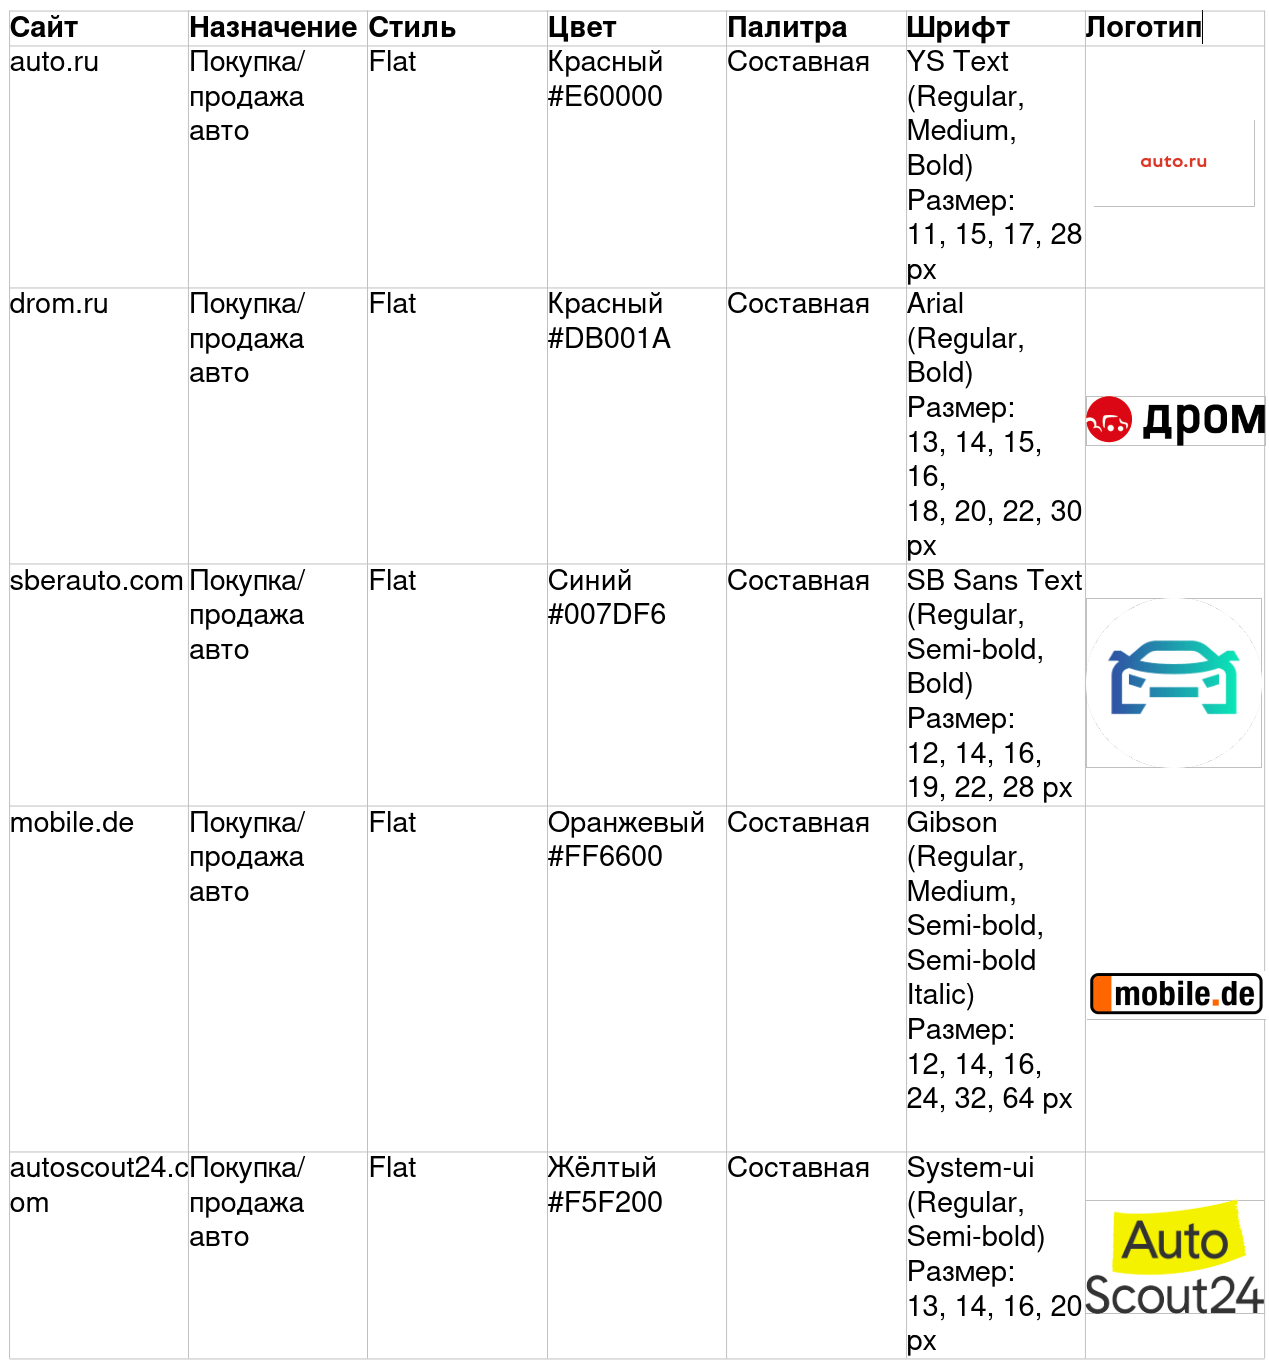
\includegraphics[width=\linewidth]{table}}
\end{minipage}
\bigskip

\noindent
\begin{minipage}{\linewidth}
    \fbox{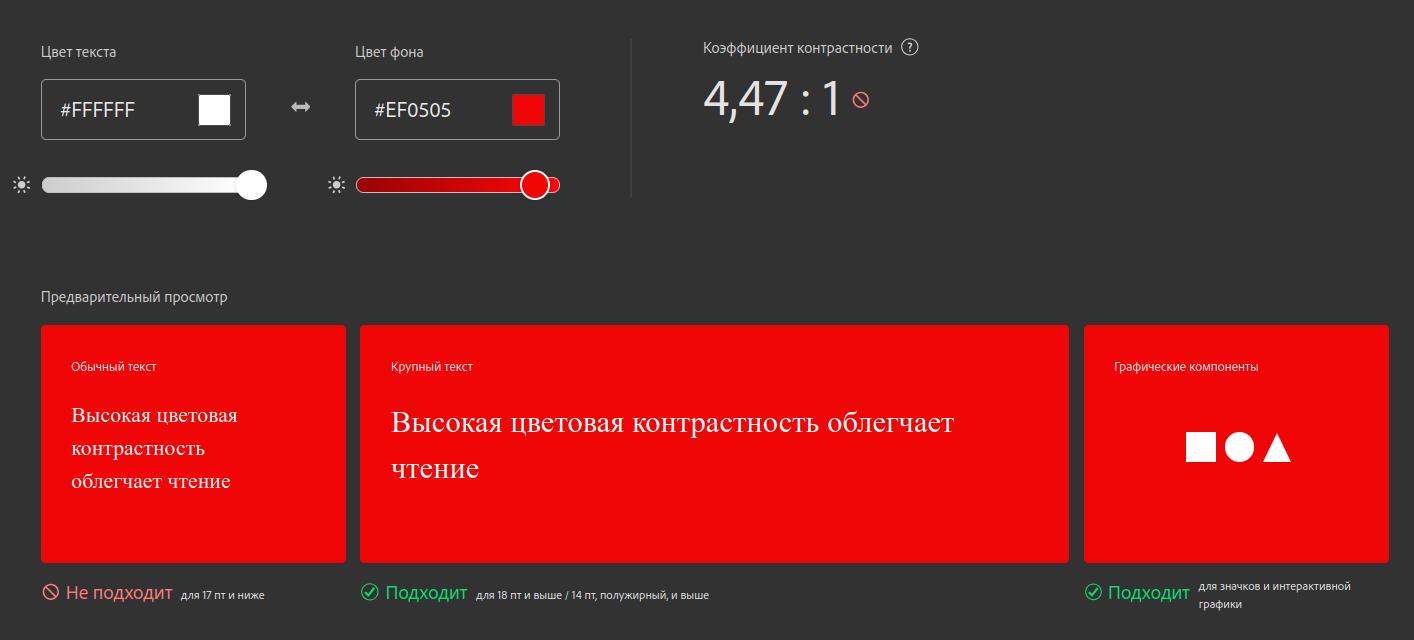
\includegraphics[width=\linewidth]{color1_before}}
    \captionof{figure}{до}
\end{minipage}
\bigskip

\noindent
\begin{minipage}{\linewidth}
    \fbox{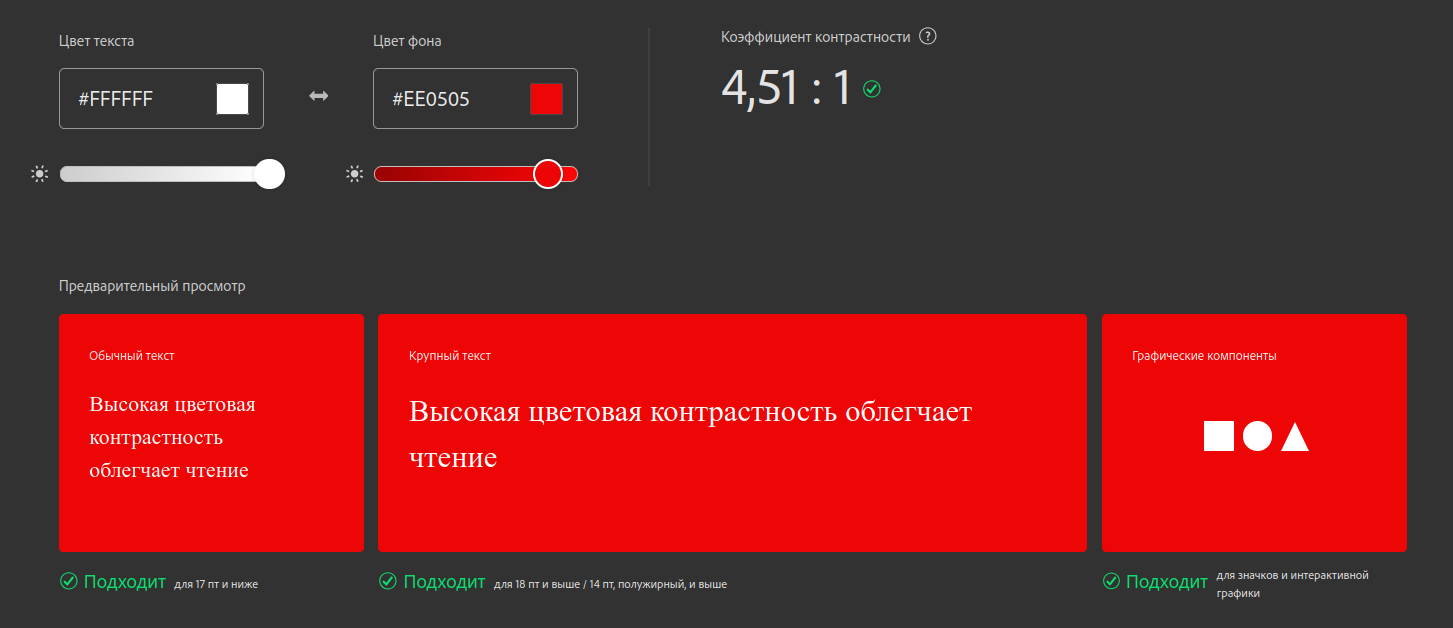
\includegraphics[width=\linewidth]{color1_after}}
    \captionof{figure}{после}
\end{minipage}
\bigskip

\noindent
\begin{minipage}{\linewidth}
    \fbox{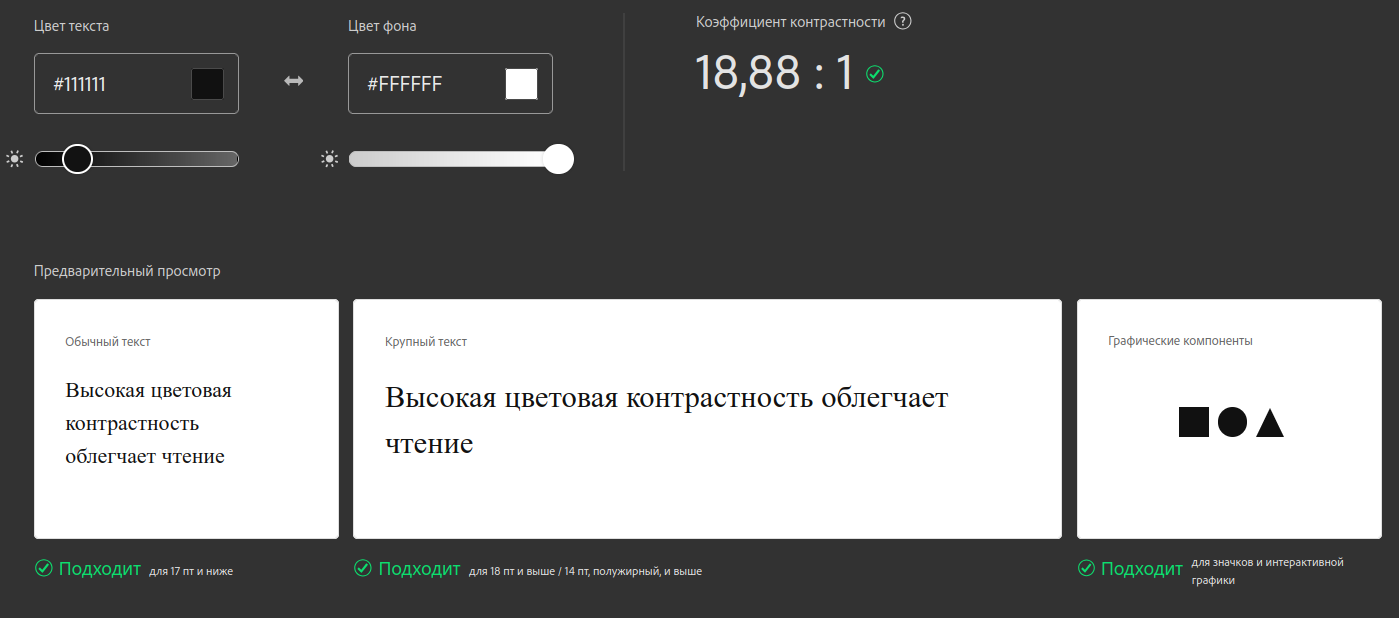
\includegraphics[width=\linewidth]{color2}}
\end{minipage}
\bigskip

\noindent
\begin{minipage}{\linewidth}
    \fbox{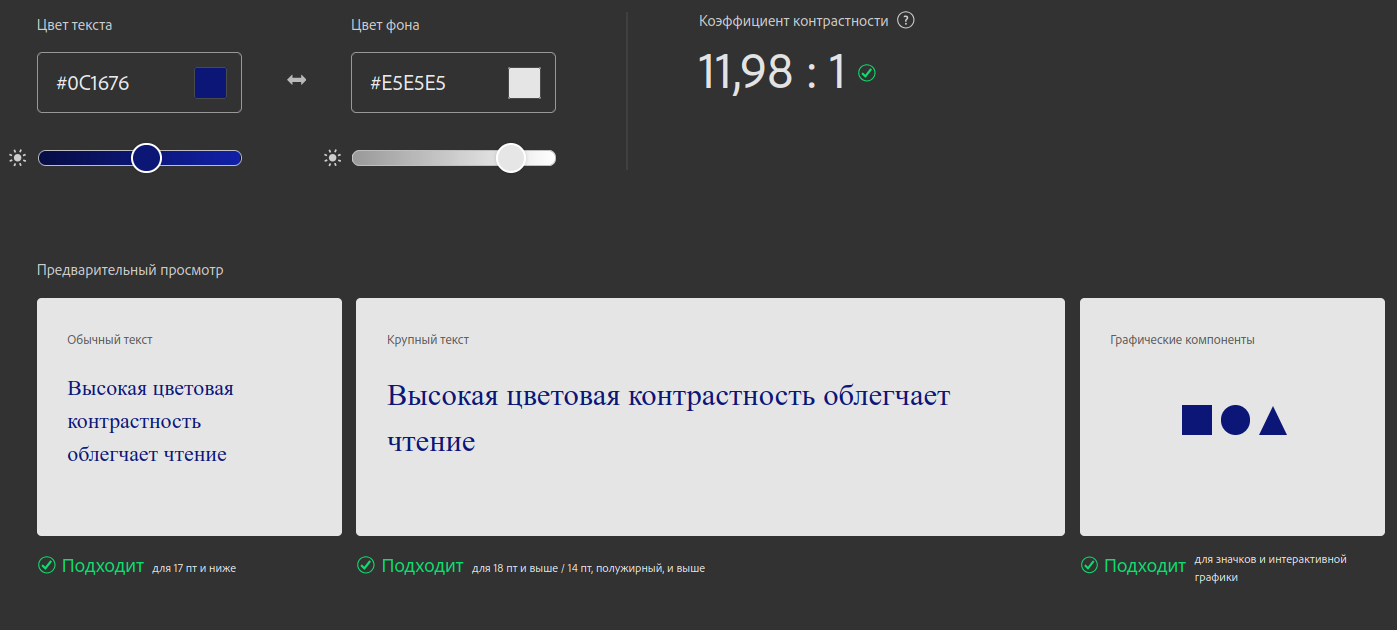
\includegraphics[width=\linewidth]{color3}}
\end{minipage}
\bigskip

\noindent
\begin{minipage}{\linewidth}
    \fbox{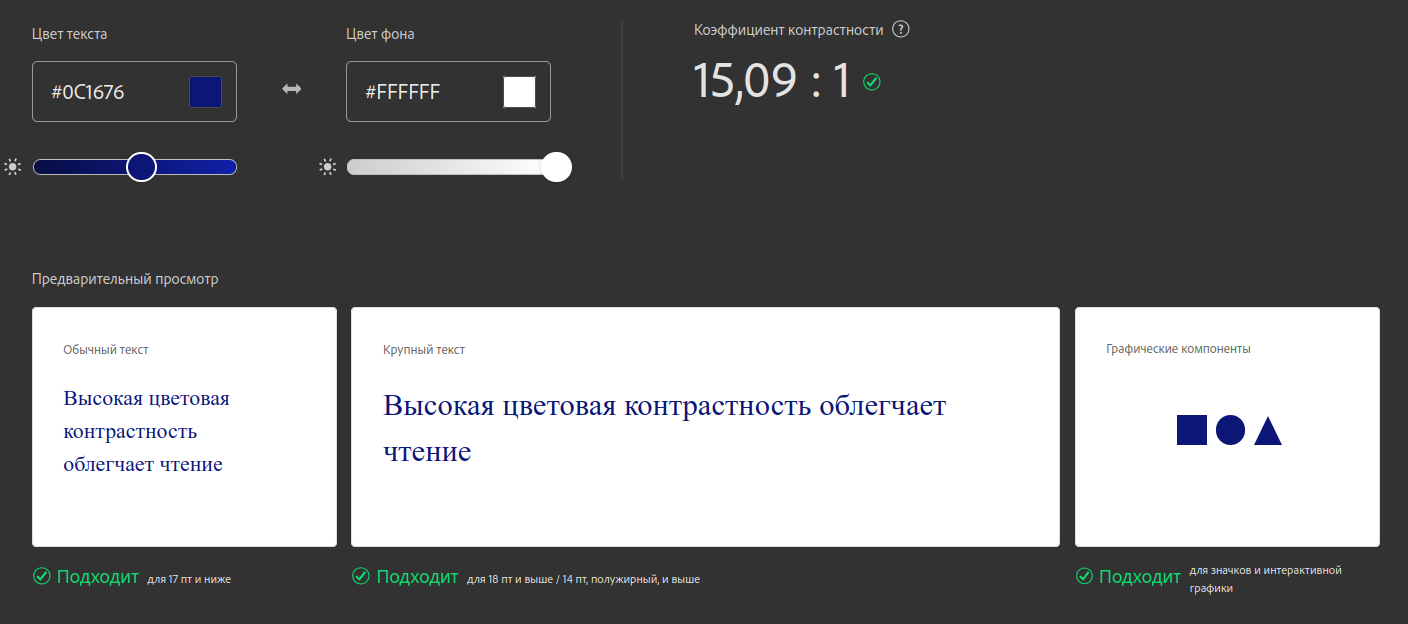
\includegraphics[width=\linewidth]{color4}}
\end{minipage}
\bigskip

\noindent
\begin{minipage}{\linewidth}
    \fbox{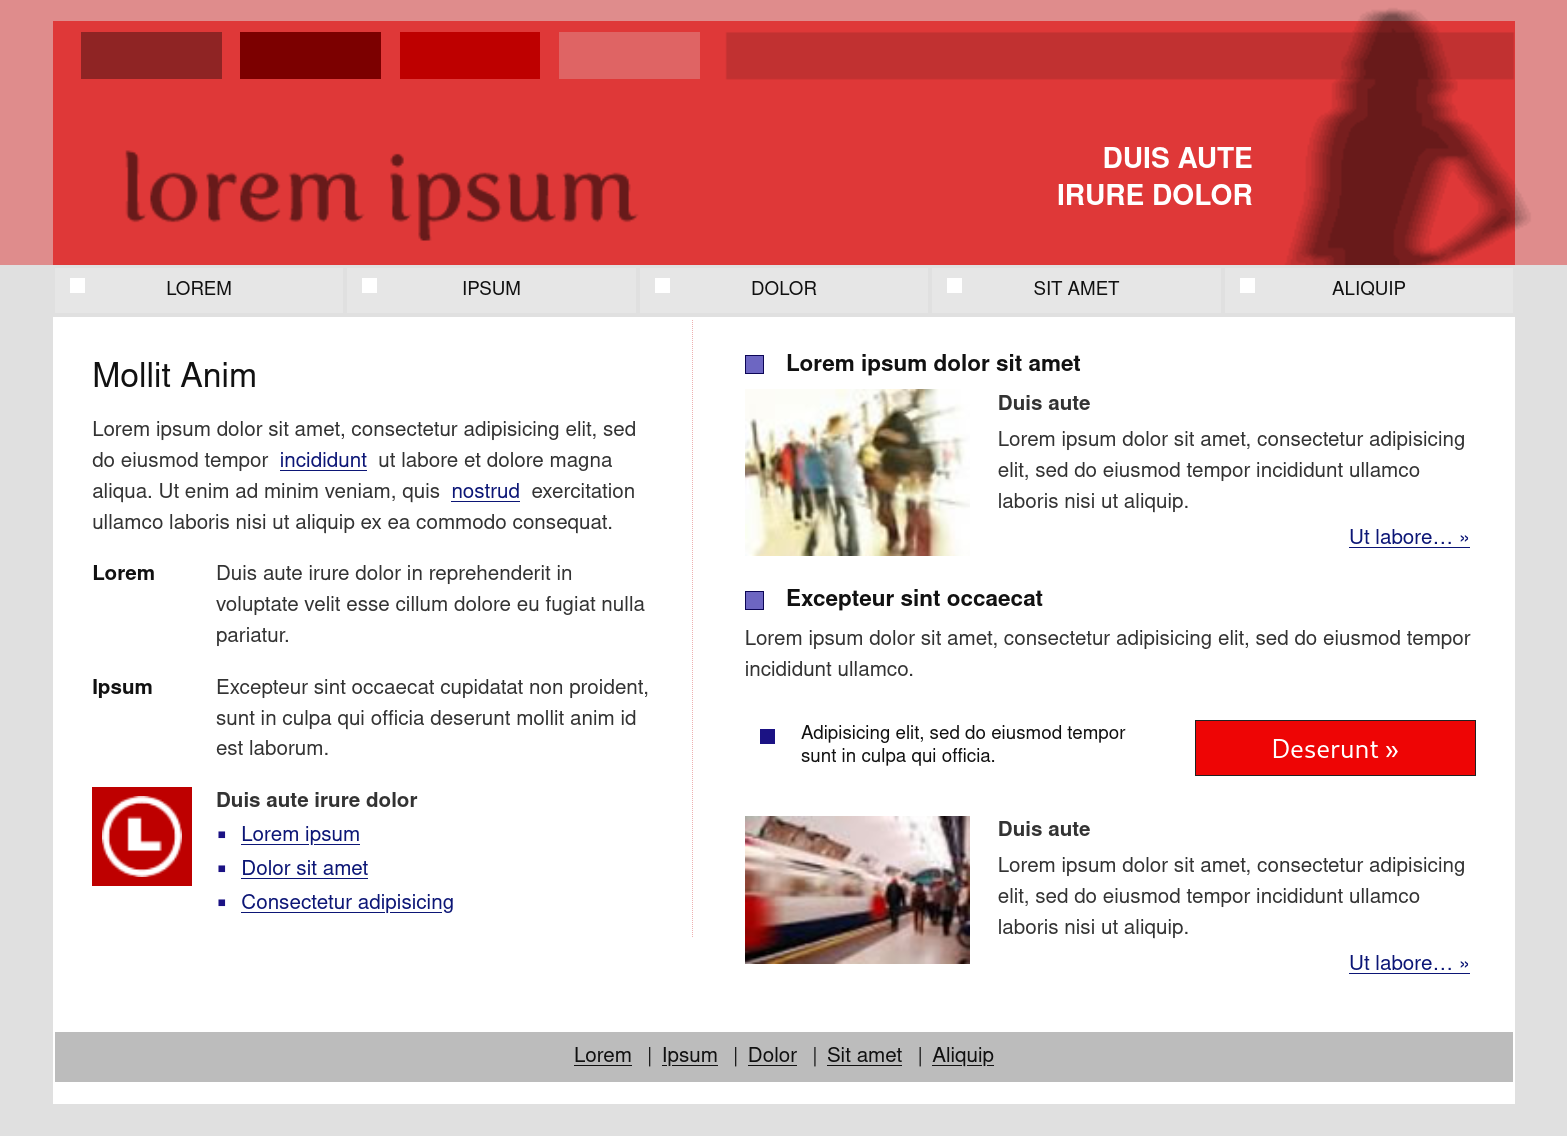
\includegraphics[width=\linewidth]{generated}}
\end{minipage}
\bigskip

\textbf{Контрольные вопросы и ответы}

\begin{enumerate}
    \item Что такое цветовая палитра для веб и какая система описания цвета используется для веб-цветов?

Цветовая палитра для веб — это набор цветов, используемых в дизайне веб-страницы или приложения. Цветовая палитра помогает создать визуальную гармонию и поддерживает идентичность бренда.

Системы описания цвета:

HEX: шестнадцатеричный код, начинающийся с символа #, например, #FFFFFF для белого.

RGB: описание цвета через значения красного, зеленого и синего (от 0 до 255), например, rgb(255, 255, 255).

HSL: цветовое пространство, описывающее цвет через оттенок, насыщенность и яркость, например, hsl(0, 100\%, 100\%).
    \item На что необходимо опираться при выборе цветовой палитры? Какие существуют рекомендации по количеству и соотношению основных цветов интерфейса?

При выборе цветовой палитры нужно учитывать:

Целевая аудитория: понимание предпочтений пользователей и их восприятия цветов.

Психология цвета: разные цвета вызывают различные эмоции и ассоциации.

Цель продукта: цвета должны соответствовать функциональности и задачам сайта или приложения.

Рекомендации по количеству и соотношению основных цветов:
используйте 1-3 основных цвета и 1-2 акцентных цвета.
Поддерживайте баланс между основными и нейтральными цветами (например, серыми или белыми) для создания контраста.
    \item Как учитываются аномалии цветовосприятия пользователей при проектировании интерфейса?

Аномалии цветовосприятия, такие как дальтонизм, могут повлиять на восприятие цветов. Для учета этих факторов используйте высокий контраст между текстом и фоном, 
избегайте использования цветовых комбинаций, которые трудно различить (например, красный и зеленый), 
используйте текстуры или узоры для обозначения различий, помимо цвета, 
предоставляйте возможность настраивать цвета интерфейса для пользователей с нарушениями цветовосприятия.
    \item Какие существуют программные средства по оптимизации цветовой палитры для веб-ресурсов?

Adobe Color, Coolors, Colorzilla, Paletton.
    \item Какие существуют рекомендации по подбору цветов интерфейса?

        Определите основную цветовую тему на основе целей вашего сайта или приложения, учитывайте доступность (Цвета должны быть различимы для всех пользователей, включая людей с нарушениями зрения), используйте инструменты для проверки контраста (например, WebAIM Contrast Checker) для проверки читабельности текста на фоне, тестируйте палитры на различных устройствах и экранах, чтобы убедиться, что цвета выглядят так, как вы ожидаете.
    \item Как можно учитывать цветовоспроизведение интерфейса на различных устройствах при выборе цветовой палитры?

Использовать стандартизированные цветовые модели (например, sRGB), чтобы обеспечить согласованность, проводить тестирование на различных экранах (мобильных, планшетах, компьютерах), чтобы увидеть, как цвета выглядят в разных условиях, учитывать, что яркость и контрастность могут варьироваться в зависимости от освещения и технологии экрана, и использовать цвета (например, серые), которые хорошо смотрятся в разных условиях.
\end{enumerate}

\end{document}
